\documentclass[journal,12pt,twocolumn]{IEEEtran}

\usepackage{setspace}
\usepackage{gensymb}

\singlespacing


\usepackage[cmex10]{amsmath}

\usepackage{amsthm}

\usepackage{mathrsfs}
\usepackage{txfonts}
\usepackage{stfloats}
\usepackage{bm}
\usepackage{cite}
\usepackage{cases}
\usepackage{subfig}

\usepackage{longtable}
\usepackage{multirow}

\usepackage{enumitem}
\usepackage{mathtools}
\usepackage{steinmetz}
\usepackage{tikz}
\usepackage{circuitikz}
\usepackage{verbatim}
\usepackage{tfrupee}
\usepackage[breaklinks=true]{hyperref}
\usepackage{graphicx}
\usepackage{tkz-euclide}

\usetikzlibrary{calc,math}
\usepackage{listings}
    \usepackage{color}                                            %%
    \usepackage{array}                                            %%
    \usepackage{longtable}                                        %%
    \usepackage{calc}                                             %%
    \usepackage{multirow}                                         %%
    \usepackage{hhline}                                           %%
    \usepackage{ifthen}                                           %%
    \usepackage{lscape}     
\usepackage{multicol}
\usepackage{chngcntr}

\DeclareMathOperator*{\Res}{Res}

\renewcommand\thesection{\arabic{section}}
\renewcommand\thesubsection{\thesection.\arabic{subsection}}
\renewcommand\thesubsubsection{\thesubsection.\arabic{subsubsection}}

\renewcommand\thesectiondis{\arabic{section}}
\renewcommand\thesubsectiondis{\thesectiondis.\arabic{subsection}}
\renewcommand\thesubsubsectiondis{\thesubsectiondis.\arabic{subsubsection}}


\hyphenation{op-tical net-works semi-conduc-tor}
\def\inputGnumericTable{}                                 %%

\lstset{
%language=C,
frame=single, 
breaklines=true,
columns=fullflexible
}
\begin{document}


\newtheorem{theorem}{Theorem}[section]
\newtheorem{problem}{Problem}
\newtheorem{proposition}{Proposition}[section]
\newtheorem{lemma}{Lemma}[section]
\newtheorem{corollary}[theorem]{Corollary}
\newtheorem{example}{Example}[section]
\newtheorem{definition}[problem]{Definition}

\newcommand{\BEQA}{\begin{eqnarray}}
\newcommand{\EEQA}{\end{eqnarray}}
\newcommand{\define}{\stackrel{\triangle}{=}}
\bibliographystyle{IEEEtran}

\providecommand{\mbf}{\mathbf}
\providecommand{\pr}[1]{\ensuremath{\Pr\left(#1\right)}}
\providecommand{\qfunc}[1]{\ensuremath{Q\left(#1\right)}}
\providecommand{\sbrak}[1]{\ensuremath{{}\left[#1\right]}}
\providecommand{\lsbrak}[1]{\ensuremath{{}\left[#1\right.}}
\providecommand{\rsbrak}[1]{\ensuremath{{}\left.#1\right]}}
\providecommand{\brak}[1]{\ensuremath{\left(#1\right)}}
\providecommand{\lbrak}[1]{\ensuremath{\left(#1\right.}}
\providecommand{\rbrak}[1]{\ensuremath{\left.#1\right)}}
\providecommand{\cbrak}[1]{\ensuremath{\left\{#1\right\}}}
\providecommand{\lcbrak}[1]{\ensuremath{\left\{#1\right.}}
\providecommand{\rcbrak}[1]{\ensuremath{\left.#1\right\}}}
\theoremstyle{remark}
\newtheorem{rem}{Remark}
\newcommand{\sgn}{\mathop{\mathrm{sgn}}}
\providecommand{\abs}[1]{\left\vert#1\right\vert}
\providecommand{\res}[1]{\Res\displaylimits_{#1}} 
\providecommand{\norm}[1]{\left\lVert#1\right\rVert}
%\providecommand{\norm}[1]{\lVert#1\rVert}
\providecommand{\mtx}[1]{\mathbf{#1}}
\providecommand{\mean}[1]{E\left[ #1 \right]}
\providecommand{\fourier}{\overset{\mathcal{F}}{ \rightleftharpoons}}
%\providecommand{\hilbert}{\overset{\mathcal{H}}{ \rightleftharpoons}}
\providecommand{\system}{\overset{\mathcal{H}}{ \longleftrightarrow}}
	%\newcommand{\solution}[2]{\textbf{Solution:}{#1}}
\newcommand{\solution}{\noindent \textbf{Solution: }}
\newcommand{\cosec}{\,\text{cosec}\,}
\providecommand{\dec}[2]{\ensuremath{\overset{#1}{\underset{#2}{\gtrless}}}}
\newcommand{\myvec}[1]{\ensuremath{\begin{pmatrix}#1\end{pmatrix}}}
\newcommand{\mydet}[1]{\ensuremath{\begin{vmatrix}#1\end{vmatrix}}}
\numberwithin{equation}{subsection}

\makeatletter
\@addtoreset{figure}{problem}
\makeatother
\let\StandardTheFigure\thefigure
\let\vec\mathbf

\renewcommand{\thefigure}{\theproblem}

\def\putbox#1#2#3{\makebox[0in][l]{\makebox[#1][l]{}\raisebox{\baselineskip}[0in][0in]{\raisebox{#2}[0in][0in]{#3}}}}
     \def\rightbox#1{\makebox[0in][r]{#1}}
     \def\centbox#1{\makebox[0in]{#1}}
     \def\topbox#1{\raisebox{-\baselineskip}[0in][0in]{#1}}
     \def\midbox#1{\raisebox{-0.5\baselineskip}[0in][0in]{#1}}
\vspace{3cm}
\title{Assignment 5}
\author{Sachinkumar Dubey - EE20MTECH11009}

\maketitle
\newpage
\bigskip
\renewcommand{\thefigure}{\theenumi}
\renewcommand{\thetable}{\theenumi}
Download all python codes from 
\begin{lstlisting}
https://github.com/sachinomdubey/Matrix-theory/Assignment5/codes
\end{lstlisting}
%
and latex-tikz codes from 
%
\begin{lstlisting}
https://github.com/sachinomdubey/Matrix-theory/Assignment5
\end{lstlisting}
\subsection{Problem}
(Geolin 1.9) $AB$ is a line-segment. $P$ and $Q$ are points on opposite sides of $AB$ such that each of them is equidistant from the points $A$ and $B$. Show that the line $PQ $ is the perpendicular bisector of $AB$.
\begin{figure}[h!]
\centering
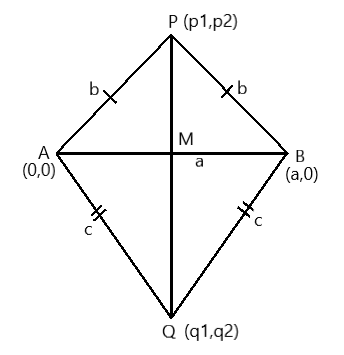
\includegraphics[width=7cm, height=7cm]{Figure_51}
\caption{}
\label{Fig4}
\end{figure}
\subsection{Explanation}
In order to prove that line $PQ $ is the perpendicular bisector of $AB$, two conditions need to be met:
\begin{enumerate}
    \item $AM$=$BM$
    \item Angle between line $AB$ and line $PQ$ should be $90\degree$.
\end{enumerate}
Steps to prove the first condition are as follow:
\begin{enumerate}
    \item Finding the normal vectors of line $PQ$. Further using the normal vector to find the equation of line $PQ$. 
    \item The solution of equation of line $AB$ and line $PQ$ will give the co-ordinates of point $M$. 
    \item Using the distance formula to prove that $AM$=$BM$.
\end{enumerate}
Steps to prove the second condition are as follow:
\begin{enumerate}
    \item Finding the normal vectors of line $AB$ and $PQ$.
    \item Taking their dot product and checking whether it is zero. If the dot product of the normal vectors is zero, the lines will be perpendicular to each other.
\end{enumerate}

\subsection{Solution}
Let the Points $\vec{A}$, $\vec{B}$, $\vec{P}$ and $\vec{Q}$ be:
\begin{align}
    \vec{A}=\myvec{0 \\ 0} & \vec{B}=\myvec{a \\ 0} & \vec{P}=\myvec{p_1 \\ p_2}&\vec{Q}=\myvec{q_1 \\ q_2}
\end{align}
The point $\vec{P}$ is equidistant from the points $\vec{A}$ and $\vec{B}$. Let the distance be $b$. Then we can write:
\begin{align}
    \norm{\vec{A}-\vec{P}}=b \label{eq2.2}\\
    \norm{\vec{B}-\vec{P}}=b \label{eq2.3}
\end{align}
The equation \ref{eq2.2} can be further written as:
\begin{align}
    \norm{\myvec{0\\0}-\myvec{p_1\\p_2}}=b \\
    \sqrt{p_1^2+p_2^2}=b\\
    p_1^2+p_2^2=b^2 \label{eq2.6}
\end{align}
Similarly, the equation \ref{eq2.3} can be further written as:
\begin{align}
    \norm{\myvec{a\\0}-\myvec{p_1\\p_2}}=b \\
    \sqrt{(a-p_1)^2+p_2^2}=b\\
    p_1^2+p_2^2-2ap_1+a^2=b^2 \label{eq2.9}
\end{align}
From equations \ref{eq2.6} and \ref{eq2.9}, we get:
\begin{align}
    p_1^2+p_2^2-2ap_1+a^2=p_1^2+p_2^2\\
    \therefore a^2-2ap_1=0\\
    \implies p_1=a/2
\end{align}
Putting $p_1$ in equation \ref{eq2.6}:
\begin{align}
   (a/2)^2+p_2^2=b^2 \\
    p_2=\pm \frac{\sqrt{4b^2-a^2}}{2}
\end{align}
Taking positive value of $p_2$ as the point $\vec{P}$ lies in the first quadrant.
\begin{align}
    \therefore p_2=\frac{\sqrt{4b^2-a^2}}{2}
\end{align}
Thus, point $\vec{P}$ is:
\begin{align}
    \vec{P}=\myvec{a/2\\\sqrt{4b^2-a^2}/2}\\
\end{align}
Similarly, The point $\vec{Q}$ equidistant from the points $\vec{A}$ and $\vec{B}$ with distance $c$ can be calculated as:
\begin{align}
    \vec{Q}=\myvec{a/2\\-\sqrt{4c^2-a^2}/2}
\end{align}
The directional vector of the line PQ is given by:
\begin{align}
    \vec{m}_{PQ}=(\vec{P}-\vec{Q})\\
    \vec{m}_{PQ}=\myvec{a/2\\\sqrt{4b^2-a^2}/2}-\myvec{a/2\\-\sqrt{4c^2-a^2}/2}\\
    \vec{m}_{PQ}=\myvec{0\\\displaystyle \frac{\sqrt{4b^2-a^2}+\sqrt{4c^2-a^2}}{2}}
\end{align}
The normal vector of line PQ is:
\begin{align}
    \vec{n}_{PQ} = \myvec{0&-1\\1&0}\vec{m}_{PQ} \\
    \vec{n}_{PQ} = \myvec{\displaystyle \frac{-\sqrt{4b^2-a^2}-\sqrt{4c^2-a^2}}{2}\\0} \label{eq3.23}
\end{align}
Equation of a line PQ in terms of normal vector is by:
\begin{align}
\vec{n}_{PQ}^T\brak{\vec{x}-\vec{P}} &= 0\\
\therefore \myvec{a/2 & 0} \vec{x} &= 0 \label{eq3.25}
\end{align}
Since the line AB is the X-axis, its equation and normal vector can be written as:
\begin{align}
\myvec{0 & 1} \vec{x} &= 0 \label{eq3.26}\\
\vec{n}_{AB}=\myvec{0\\1} \label{eq3.27}
\end{align}
Solving equation \ref{eq3.25} and \ref{eq3.26}, we get the cordinates of point $\vec{M}$:
\begin{align}
    \vec{M}=\myvec{a/2\\0}
\end{align}
The segments $AM$ and $BM$ are given as:
\begin{align}
    AM=\norm{\vec{A}-\vec{M}} \\
    \therefore AM=\norm{\myvec{0\\0}-\myvec{a/2\\0}}\\
    \therefore AM=\sqrt{a^2/4+0}=a/2 \label{eq3.30}\\
    Similarly,BM=\norm{\vec{B}-\vec{M}} \\
    \therefore BM=\norm{\myvec{a\\0}-\myvec{a/2\\0}}\\
    \therefore BM=\sqrt{a^2/4+0}=a/2\label{eq3.33}
\end{align}
From equation \ref{eq3.30} and \ref{eq3.33} :
\begin{align}
    AM=BM \label{eq3.35}
\end{align}
Using equation \ref{eq3.23} and \ref{eq3.27}, dot product of normal vectors of line $AB$ and $PQ$ is:
\begin{align}
    \vec{n}_{AB}^T\vec{n}_{PQ}=\myvec{0&1}\myvec{\displaystyle \frac{-\sqrt{4b^2-a^2}-\sqrt{4c^2-a^2}}{2}\\0}\\
    \therefore\vec{n}_{AB}^T\vec{n}_{PQ}=0 \label{eq3.37}
\end{align}
From equation \ref{eq3.35} and \ref{eq3.37}, $PQ$ is perpendicular bisector of $AB$. Hence proved.
\end{document}